\documentclass[12pt,oneside]{fithesis}
%\documentclass[12pt,draft,oneside]{fithesis}
\usepackage[utf8]{inputenc}
\usepackage[IL2]{fontenc}
\usepackage[plainpages=false, pdfpagelabels]{hyperref}
\usepackage{paralist}
\usepackage{graphicx}
\usepackage{amsmath}
\usepackage{color}
\usepackage{courier}
\usepackage[czech]{babel}

\usepackage{float}
\floatstyle{ruled}

\thesistitle{Solventnost pojišťovny}
\thesissubtitle{Seminární práce}
\thesisstudent{Marek Bryša}
\thesiswoman{false}
\thesisfaculty{sci}
\thesislang{cz}
\thesisyear{jaro 2012}

\begin{document}
\FrontMatter
\ThesisTitlePage


\MainMatter
\tableofcontents
\chapter{Úvod}
%http://www.skvara.cz/__cw_files/poji%C5%A1t%C4%9Bn%C3%AD/solvencyII/.10/.07/.abe645bf575778fda76cc843d938629e1150540710/SolvencyII.doc
%VZ: ciste pojistne PDF:134
%vl k 67
Solventnost pojišťovny znamená její schopnost plnit stanovené neznámé budoucí závazky. Pokud aktiva pojišťovny nedosahují potřebné výše nebo z jiných důvodů není schopna nároky plnit, řekneme, že není solventní.

Existují obecná kritéria solventností stanovená Evropskou komisí, která zohledňují tyto faktory:
\begin{compactitem}
\item velikost pojišťovny a její vlastní dluh
\item poskytované pojistné produkty na trhu, územní působnost
\item efektivitu činnosti managementu vyjádřenou rozsahem
škodních událostí, kontrolou výdajů a kvalitou prodeje
\item riziko nelikvidovaných škod přesahujících vytvořené technické
rezervy
\item negativní dopady růstu míry inflace
\item stupeň vystavení se riziku změny směnného kurzu
\item základy oceňování aktiv a pasiv
\end{compactitem}
Dohled v České republice se řídí především vyhláškou ČNB č. 434/2009, kde jsou také v přílohách uvedeny příslušné výpočetní vzorce. Naneštěstí je není možno aplikovat na veřejně přístupná data, která pojišťovny poskytují. 

Při krytí závazků řeší pojišťovny zejména tyto situace:
\begin{compactitem}
\item Potřebu okamžité likvidity pro krytí závazků způsobených událostmi v během daného roku.
\item Tvorbu dostatečných technických rezerv, které slouží ke krytí závazků, které budou řešeny v budoucnosti.
\item Vytváření dalších rezerv pro případ mimořádných výdajů.
\end{compactitem}
\section{Solvency II}
Regulační systém Solvency II vznikl jako směrnice Evropského parlamentu a Rady 2009/138/ES ze dne 25. listopadu 2009 o přístupu k pojišťovací a zajišťovací činnosti a jejím výkonu. Navazuje na regulační opatření bank Basel II. Je plánováno, že bude plně implementován do roku 2014. Základem jsou následující 3 pilíře.
\subsection{Kvantifikace}
První pilíř se zabývá kvantitativními požadavky, včetně technických rezerv a kapitálových nároků. Definuje 2 kapitálových požadavků:
\begin{itemize}
\item{\textbf{MCR -- minimální kapitálové požadavky}} Jsou kalibrovány na 85\% pravděpodobnost kapitálové přiměřenosti za rok. Porušení znamená intervenci dohledového orgánu.
\item{\textbf{SCR -- solventnostní kapitálové požadavky}} Znamenají, že pojišťovna s 99.5\% pravděpodbností během roku splní své závazky. Vlastní kapitál musí být vyšší než SCR.
\end{itemize}
\subsection{Řízení rizika, management}
Požaduje zavedení důsledných procesů řízení zejména těchto rizik:
\begin{compactitem}
\item pojistné riziko
\item tržní riziko
\item kreditní riziko
\item operační riziko
\item riziko z nesouladu při alokaci aktiv a pasiv
\end{compactitem}
\subsection{Zveřejnění informací}
Třetí pilíř se zabývá hlášením a zveřejňováním informací, které mají vést k vyšší transparentnosti. Údaje o solventnosti a finanční stabilitě by měly být uveřejněný každý rok ve své úplnosti. Konkurenční prostředí by mělo vynutit vyšší standardy solventnosti.
\chapter{Poměrové ukazatele}
\footnote{Převzato z Růčková: Finanční analýza : metody, ukazatele, využití v praxi, 2.aktualizované vydání, Praha: GRADA Publishing, 2008, ISBN 978-80-247-2481-2, str. 48-50 a Grünwald, Holečková: Finanční analýza a plánování podniku, 1.vydání, Praha: Ekopress, 2007, ISBN 978-80-86929-26-2, str.112-115} Základní metodou analyzování a vykazování solventnosti pojišťovny je série následujících
poměrových ukazatelů vycházející z účetnictví pojišťovny.
\[
	\text{solvency ratio} =\frac{\text{ volný kapitál pojistitele}}{\text{čisté pojistné}}
\]

Solvency ratio neboli ukazatel solventnosti je základním účetním vyjádřením schopnosti
pojišťovny pokrýt své závazky. Volný kapitál jsou prostředky, kterými může pojišťovna
volně disponovat. Čisté pojistné je hodnota pojistného připadající na vrub pojistitele. Hodnota tohoto ukazatele by se měla pohybovat v rozmezí 30 až 50\%.
\[
	\text{retention ratio} =\frac{\text{netto pojistné}}{\text{brutto pojistné}}
\]

Stanovení netto pojistného vychází z teoretického modelu principu ekvivalence, kdy se do
rovnosti pokládají budoucí pojistné závazky a pojistné, které za pokrytí rizik platí pojištění. Brutto neboli hrubé pojistné pak představuje netto pojistné rozšířené o zahrnutí nákladových složek a zisku pojišťovny, které z daného obchodního vztahu vyplívají. Nákladovou složkou rozumíme tzv. správní náklady, které dále členíme na získávací, běžné, inkasní a náklady při výplatě důchodu. Získávací náklady jsou spjaty s mechanismy vynaložené na získání klienta formou pojistné smlouvy ohledně pojistného produktu. Běžné správní nálady jsou vynuceny převážně administrativou a provozními náklady pojištění. Inkasní složka je charakterizována výdaji vzniklými z finančních toků plynoucích z jednotlivých pojistných. Ukazatel je tak vždy menší než-li jedna, neboť netto pojistné dosahuje menších hodnot než-li brutto. Lze jej interpretovat také jakožto ukazatel efektivnosti nákladových složek. Z hlediska likvidity stanovuje, jaká část případných závazků je pokryta běžnými finančními zdroji pojišťovny.
\[
	\text{liquidity ratio} =\frac{\text{likvidní aktiva}}{\text{technické rezervy}}
\]

Poměr likvidních aktiv ku technickým rezervám vyjadřuje, do jaké míry jsou závazky
pojišťovny vyplívající z pojistných vztahů pokryty převážně peněžními prostředky. Tento
ukazatel by se dal připodobnit k indikátoru peněžní likvidity obecné finanční analýzy. Čím
vyšší hodnota liquidity ratio, tím nižší mírou likvidního rizika je pojišťovna vystavena. Na druhou stranu vysoké ukazatele likvidity obecně snižují efektivnost celkového podnikání;
ukazatel technických rezerv = technické rezervy + vlastní kapitál / čisté pojistné
ukazatel technických rezerv (technical coverage ratio ) bývá často modifikován i do podoby
poměru, kdy se v čitateli spolu s průměrným stavem technických rezerv přičítá i průměrný
stav vlastního kapitálu. Hodnota indikátoru by se měla pohybovat v rozmezí 100 až 150\%.
\[
	\text{expenses ratio} =\frac{\text{pořizovací náklady} + \text{režijní náklady}}{\text{brutto pojistné}}
\]

Expenses ratio je nákladovým ukazatelem, a jeho podoba se blíží převrácené hodnotě obratovosti nákladů ve finanční analýze běžných podniků, brutto pojistné lze totiž přirovnat k tržbám podniku. Pořizovací a režijní náklady jsou spjaty se získáním pojištění, údržbou pojistných vztahů a provozem pojišťovny.

\chapter{Příklady}
Následující tabulky byly převzaty z výročních zpráv pojišťoven za rok 2011. Vypočítáme výše uvedené poměrové ukazatele, pokud to dostupná data dovolí. U České pojištovny byl navíc ukazatel technických rezerv rozdělen na životní a neživotní složku (vlastní kapitál byl rozdělen podle poměru čistého pojistného).
\section{Česká pojišťovna}
Česká pojišťovna je s 25,1\% podílu na pojistném největší pojišťovnou na českém trhu v oblasti životního i neživotního pojišťení.\\
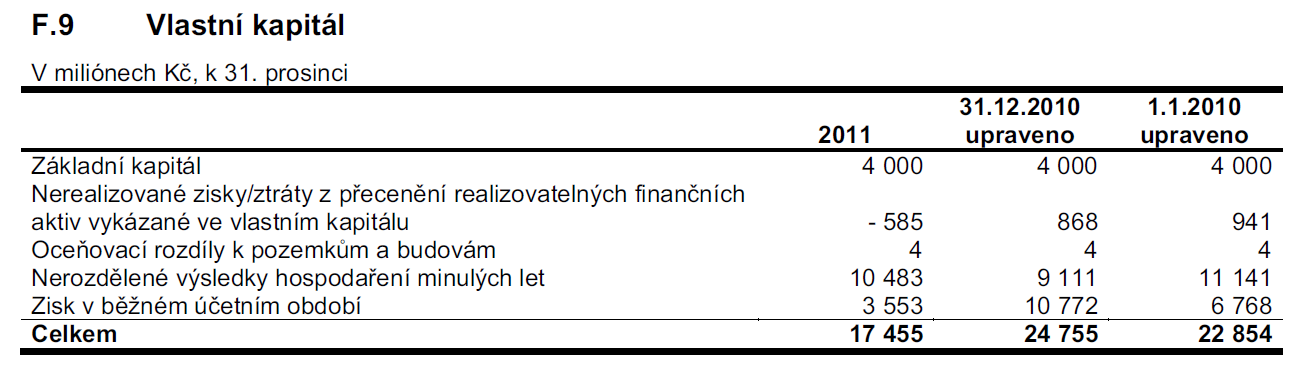
\includegraphics[width=1.0\textwidth]{cp-vlk.png}
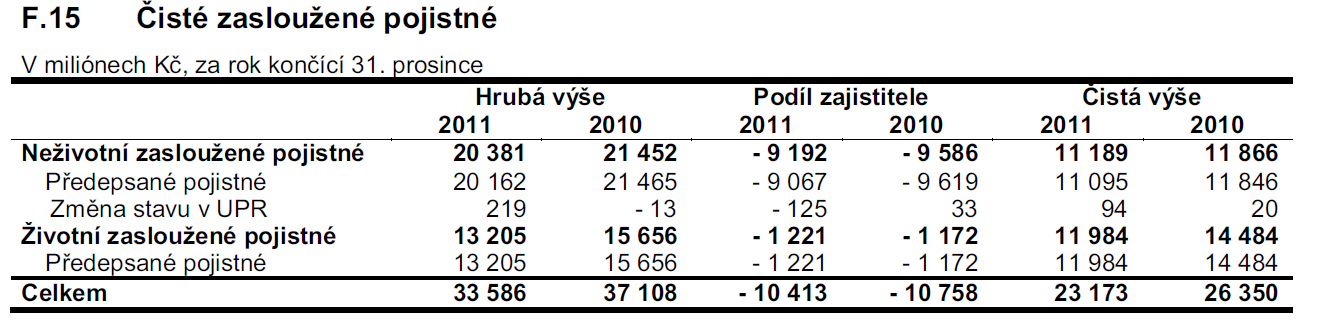
\includegraphics[width=1.0\textwidth]{cp-poj.png}
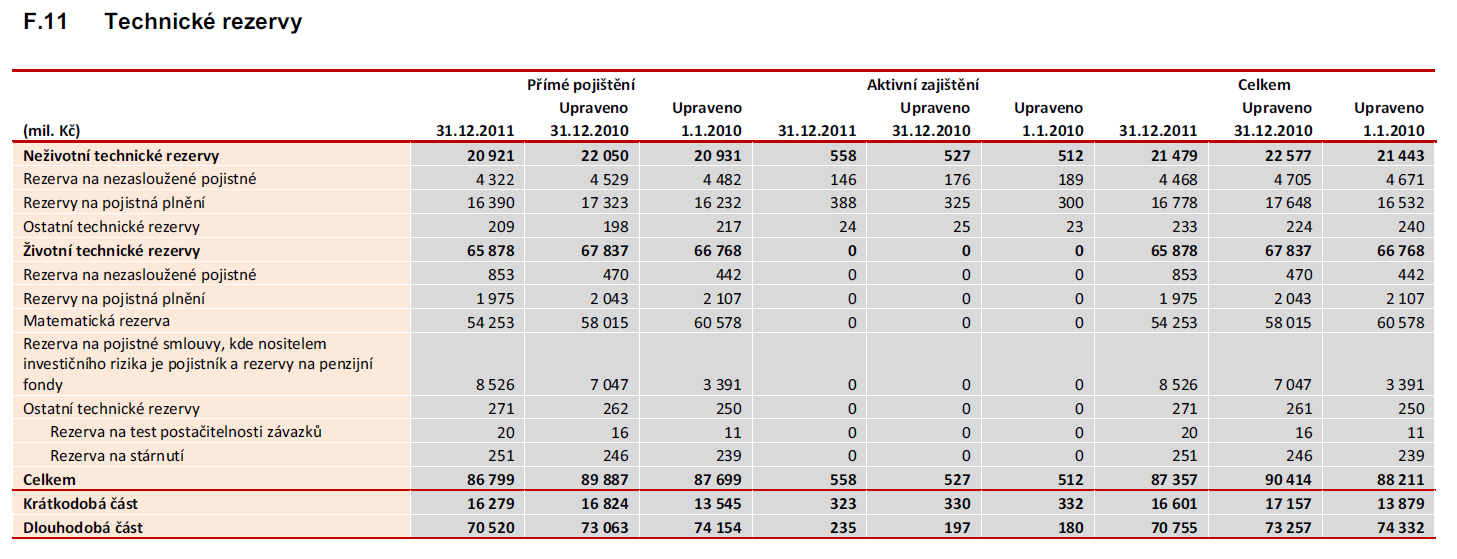
\includegraphics[width=1.0\textwidth]{cp-tr.png}
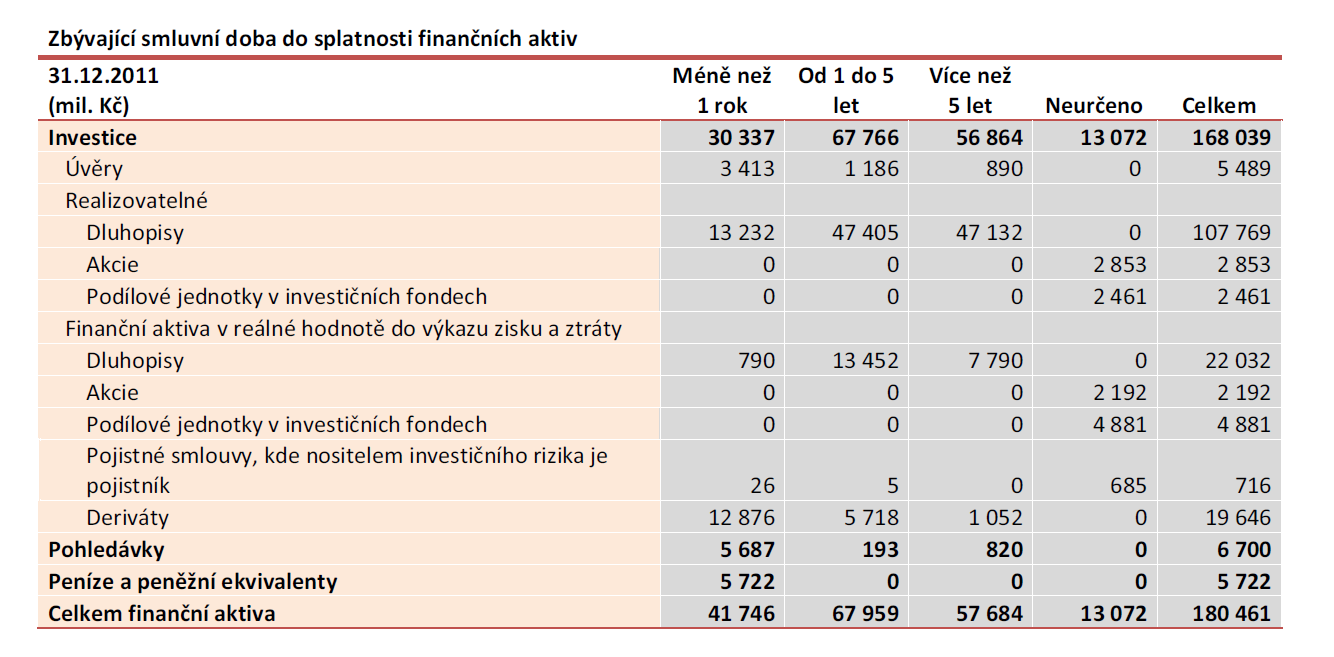
\includegraphics[width=1.0\textwidth]{cp-likv.png}
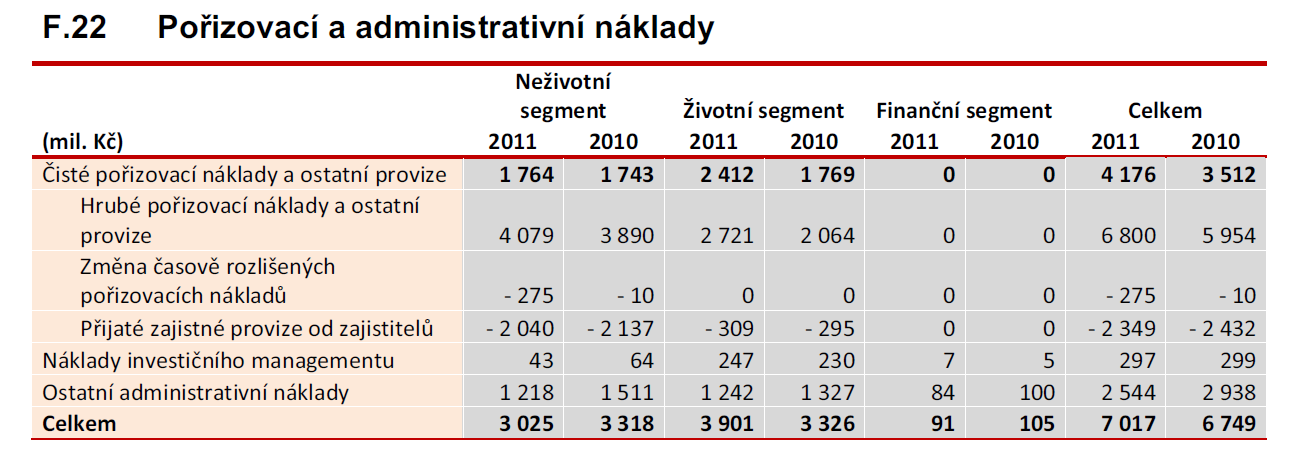
\includegraphics[width=1.0\textwidth]{cp-nakl.png}
\begin{align*}
	\text{solvency ratio}&=\frac{17 455-4 000}{23 173}=0.5806\\
	\text{ukazatel TR}&=\frac{87 357+17 455}{23 173}=4.5230\\
	\text{ukazatel TR NŽP}&=\frac{21479+17 455\cdot\frac{11189}{23173}}{11189}=2.6729\\
	\text{ukazatel TR ŽP}&=\frac{65876+17 455\cdot\frac{11984}{23173}}{11984}=6.2502\\
	\text{retention ratio}&=\frac{33586-4176}{33 586}=0.8756\\
	\text{liquidity ratio}&=\frac{41 764}{87 357}=0.4778\\
	\text{expenses ratio}&=\frac{7 017}{33 586}=0.2089\\
\end{align*}
\section{Allianz pojišťovna}
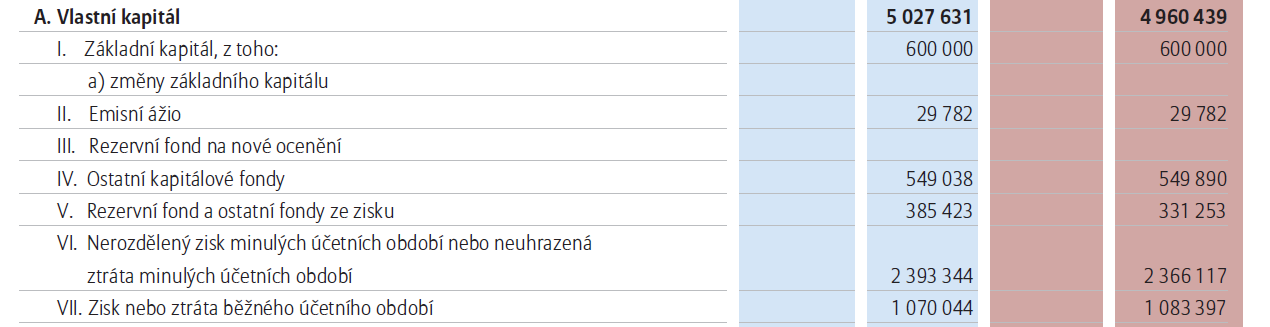
\includegraphics[width=1.0\textwidth]{al-vlk.png}
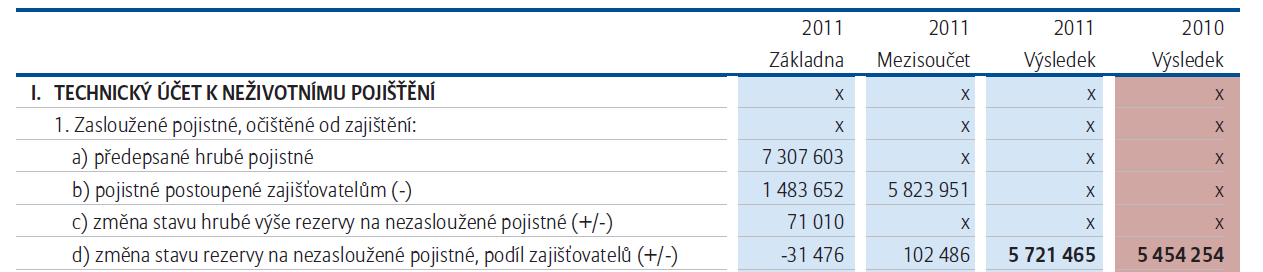
\includegraphics[width=1.0\textwidth]{al-poj1.png}
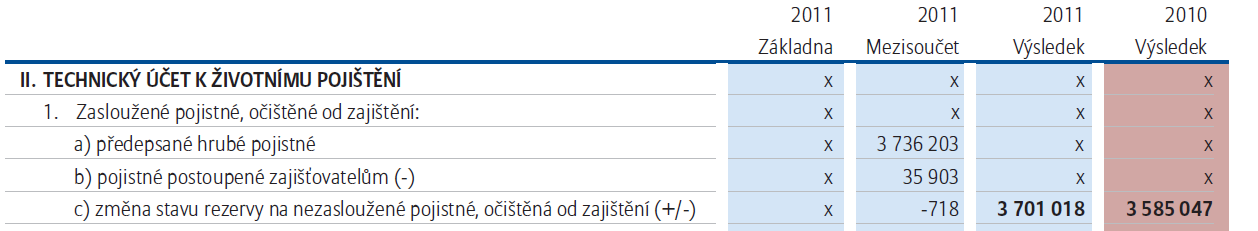
\includegraphics[width=1.0\textwidth]{al-poj2.png}

\includegraphics[width=1.0\textwidth]{al-tr.png}
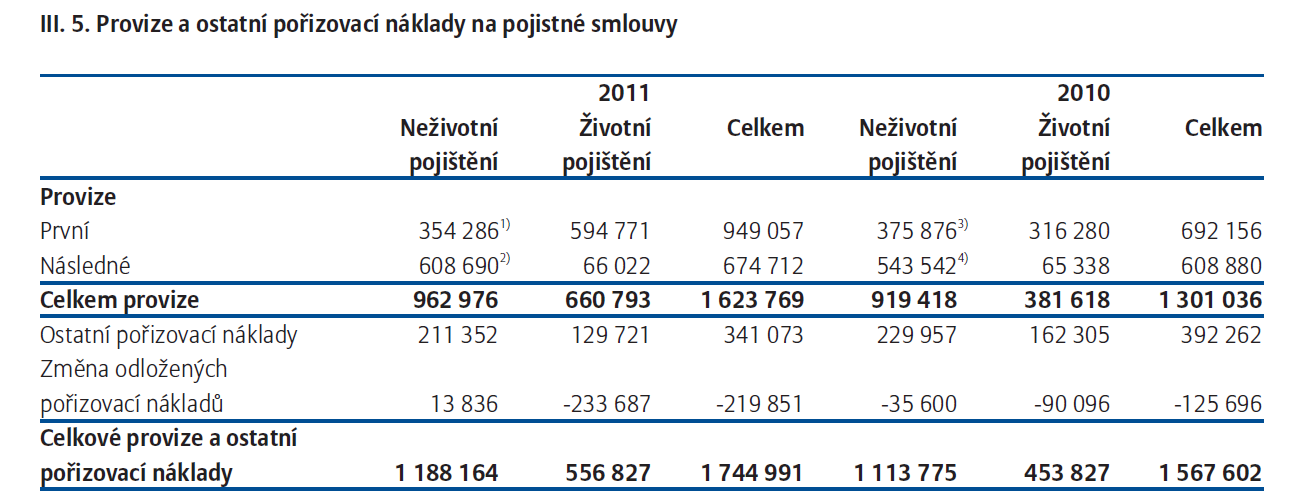
\includegraphics[width=1.0\textwidth]{al-nakl1.png}
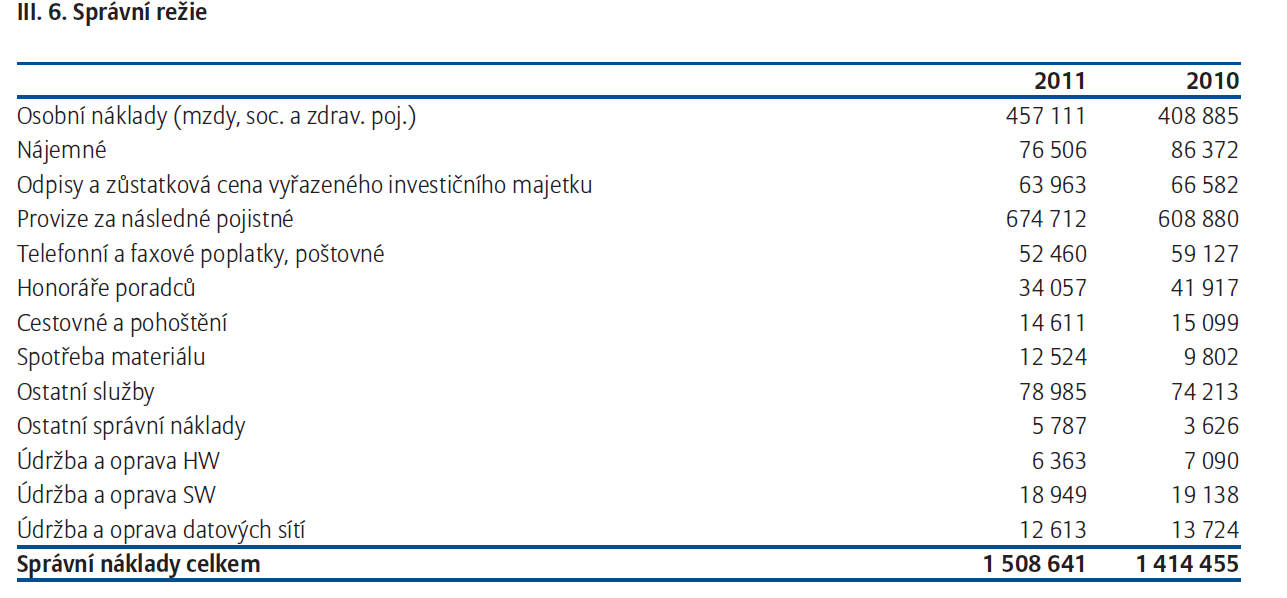
\includegraphics[width=1.0\textwidth]{al-nakl2.png}
\begin{align*}
	\text{čisté pojistné}&=5827+3701=9524\\
	\text{solvency ratio}&=\frac{5027-600}{9524}=0.4648\\
	\text{ukazatel TR}&=\frac{14322+5027}{9524}=2.0316\\
	\text{retention ratio}&=\frac{11044-1576}{11044}=0.8581\\
	\text{expenses ratio}&=\frac{1744+1508}{11044}=0.2944\\
\end{align*}
\section{Závěr}
Ukazatel solventnosti obou zkoumaných pojišťoven je významně nad 30\%, což je doporučovaná spodní hranice. Výše technických rezerv je několikanásobkem čistého pojistného. Při rozdělení na životní a neživotní složku vidíme, že u životního pojištění u České pojišťovny dosahuje tento násobek více než 6. To lze vysvětlit tím, že mnoho smluv životního pojištění ješte nebylo vyplaceno, kvůli tomu, že český pojišťovací sektor je poměrně mladý. Lze předpokládat, že na vyspělejších trzích tomu tak nebude. Nákladovost dosahuje 20 až 30 \%. Ze sledovaných ukazatelů lze říci, že Česká pojišťovna je solventnější než Allianz pojišťovna.

\begin{thebibliography}{9}

\bibitem{gretl}
Ing. František Řezáč, Ph.D., Učební materiály k předmětu Matematicko-statistické metody v pojišťovnictví, 2012
\bibitem{epstein}
Česká pojišťovna, Výroční zpráva za rok 2011
\bibitem{gilbert}
Allianz pojišťovna, Výroční zpráva za rok 2011
\bibitem{koop}
Delloite, Intro to Solvency II, February 2011
\bibitem{mankiw}
Směrnice Evropského parlamentu a Rady 2009/138/ES ze dne 25. listopadu 2009 o přístupu k pojišťovací a zajišťovací činnosti a jejím výkonu
\end{thebibliography}
\end{document}